\documentclass[noinstructornotes]{ximera}
%handout:  for handout version with no solutions or instructor notes
%handout,instructornotes:  for instructor version with just problems and notes, no solutions
%noinstructornotes:  shows only problem and solutions

%% handout
%% space
%% newpage
%% numbers
%% nooutcomes

%I added the commands here so that I would't have to keep looking them up
%\newcommand{\RR}{\mathbb R}
%\renewcommand{\d}{\,d}
%\newcommand{\dd}[2][]{\frac{d #1}{d #2}}
%\renewcommand{\l}{\ell}
%\newcommand{\ddx}{\frac{d}{dx}}
%\everymath{\displaystyle}
%\newcommand{\dfn}{\textbf}
%\newcommand{\eval}[1]{\bigg[ #1 \bigg]}

%\begin{image}
%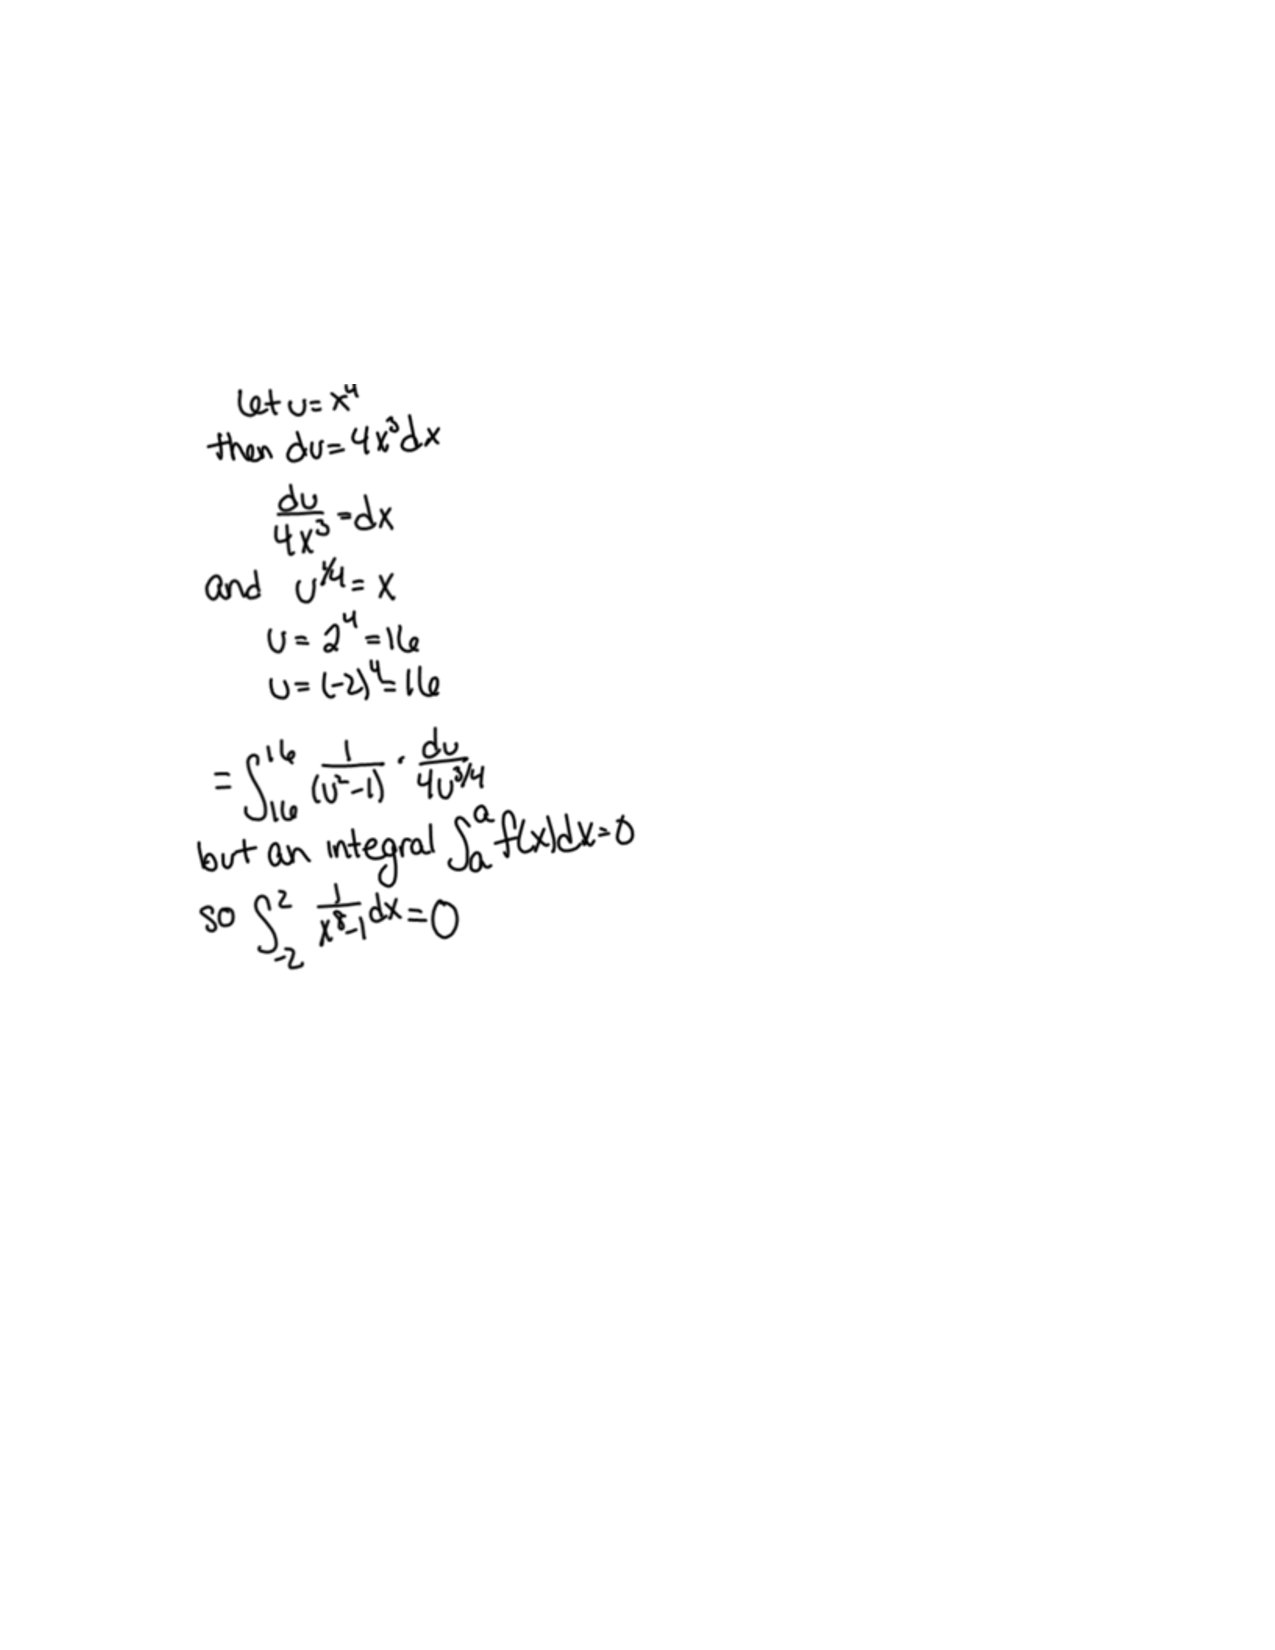
\includegraphics[trim= 170 420 250 180]{Figure1.pdf}
%\end{image}

%add a ``.'' below when used in a specific directory.
\newcommand{\RR}{\mathbb R}
\renewcommand{\d}{\,d}
\newcommand{\dd}[2][]{\frac{d #1}{d #2}}
\renewcommand{\l}{\ell}
\newcommand{\ddx}{\frac{d}{dx}}
\newcommand{\dfn}{\textbf}
\newcommand{\eval}[1]{\bigg[ #1 \bigg]}

\usepackage{multicol}

\renewenvironment{freeResponse}{
\ifhandout\setbox0\vbox\bgroup\else
\begin{trivlist}\item[\hskip \labelsep\bfseries Solution:\hspace{2ex}]
\fi}
{\ifhandout\egroup\else
\end{trivlist}
\fi} %% we can turn off input when making a master document

\title{Section 7.5: Partial Fractions}  

\begin{document}
\begin{abstract}		\end{abstract}
\maketitle



\section{Warm up:}
\begin{problem}
Give the general partial fraction decomposition for the following function.  DO NOT SOLVE FOR THE CONSTANTS! $$f(x) = \dfrac{4x^3-7}{x^6-x^2}$$

\begin{freeResponse}
	Factor the expression completely:

$$ \dfrac{4x^3-7}{x^6-x^2}= \dfrac{4x^3-7}{x^2(x^4-1)} = \dfrac{4x^3-7}{x^2(x^2-1)(x^2+1)} =\dfrac{4x^3-7}{x^2(x+1)(x-1)(x^2+1)}$$

\vspace{2mm}

Noting that the term $x^2$ is a \emph{\underline{repeated linear factor}}, we have:
$$\boxed{f(x) = \dfrac{A}{x}+\dfrac{B}{x^2}+\dfrac{C}{x+1} +\dfrac{D}{x-1} + \dfrac{Ex+F}{x^2+1}}$$
	
\end{freeResponse}

\end{problem}	

Remember that the $x^2$ term must be treated as a repeated linear factor, not as an irreducible quadratic!  Do \textbf{NOT} write the expression in \color{red} red  below\color{black}: $$f(x) = \color{red} \dfrac{Ax+B}{x^2} \color{black}+\dfrac{C}{x+1} +\dfrac{D}{x-1} + \dfrac{Ex+F}{x^2+1}$$







\section{Group work:}



%problem 1
\begin{problem}
Without determining the coefficients, write the partial fraction decomposition of the following rational function:
	\[
	\frac{5x^{13} - 6x^{12} + 7x^3 - 5x - 18}{(2x-3)(5x+9)^3 (x^2+9x+19)(x^2+9x+21)^2}
	\]
	\begin{freeResponse}
	The degree of the numerator is $13$, whereas the degree of the denominator is $10$.  
	So if we perform long division, we will get a degree $13-10=3$ polynomial plus partial fractions for the remainder term:
		\begin{align*}
		&\frac{5x^{13} - 6x^{12} + 7x^3 - 5x - 18}{(2x-3)(5x+9)^3 (x^2+9x+19)(x^2+9x+21)^2} = Ax^3 + Bx^2 + Cx + D  \\
		&+ \frac{E}{2x-3} + \frac{F}{5x+9} + \frac{G}{(5x+9)^2} + \frac{H}{(5x+9)^3} + \frac{I}{x-i_1} + \frac{J}{x-i_2}  \\
		&+ \frac{Kx+L}{x^2+9x+21} + \frac{Mx+N}{(x^2+9x+21)^2}.
		\end{align*}
		
	\dfn{Explanation of $i_1$ and $i_2$:} 
	The quadratic $x^2+9x+19$ can be factored over the real numbers, since the discriminant $b^2-4ac = 81-76 > 0$.  
	The numbers $i_1$ and $i_2$ are the two real roots to this polynomial, ie
		\[
		i_1 = \frac{-9+\sqrt{5}}{2}	\qquad	i_2=\frac{-9 - \sqrt{5}}{2}.
		\]
	Note that the polynomial $x^2+9x+21$ is irreducible (over the real numbers) since its discriminant is less than $0$.  
	\end{freeResponse}
	
\end{problem}

\begin{instructorNotes}
Make sure that the students do not attempt to perform the long division.  
We are only looking for the \dfn{form} of the decomposition, which will be a cubic polynomial followed by a sum of rational functions.  
Note that $x^2 + 9x +19$ can be factored over the reals while $x^2 + 9x + 21$ cannot.  
This is a good time to talk about the descriminant.
\end{instructorNotes}







%problem 2
\begin{problem}
Evaluate:
	\[
	\int \frac{7x^3 + 18x + 9}{x^4 + 9x^2} \d x
	\]
{\it Hint:  If $f(x) = 7x^3 + 18x + 9$, then $f(2) = 101$, $f(1) = 34$, and $f(-1) = -16$.}
	\begin{freeResponse}
	First factor the denominator
		\[
		x^4 + 9x^2 = x^2(x^2 + 9).
		\]
	The we can decompose the integrand as a partial fraction
		\begin{equation*}
		\frac{7x^3+18x+9}{x^2(x^2+9)} = \frac{A}{x} + \frac{B}{x^2} + \frac{Cx+D}{x^2+9}
		\end{equation*}
		\begin{align*}
		\Longrightarrow	\quad	7x^3 + 18x + 9 &= Ax(x^2+9) + B(x^2+9) + (Cx+D)x^2  \\
		&= Ax^3 + 9Ax + Bx^2 + 9B + Cx^3 + Dx^2  \\
		&= (A+C)x^3 + (B+D)x^2 + 9Ax + 9B.
		\end{align*}
	By equating coefficients for powers of $x$ we have that
		\begin{align*}
		&9 = 9B 	\qquad	\Longrightarrow	\qquad	B = 1  \\
		&18=9A 	\qquad	\Longrightarrow	\qquad	A = 2  \\
		&0 = B+D 	\qquad	\Longrightarrow	\qquad	0 = 1 + D 	\qquad \Longrightarrow \qquad D = -1  \\
		&7=A+C 	\qquad	\Longrightarrow	\qquad	7=2+C 	\qquad \Longrightarrow \qquad C = 5.
		\end{align*}
	Thus
		\begin{align*}
		\int \frac{7x^3 + 18x + 9}{x^4 + 9x^2} \d x
		&= \int \left( \frac{2}{x} + \frac{1}{x^2} + \frac{5x-1}{x^2+9} \right) \d x  \\
		&= 2 \ln |x| - \frac{1}{x} + 5 \int \frac{x}{x^2 + 9} \d x - \int \frac{1}{x^2 + 9} \d x  \\
		&= 2 \ln |x| - \frac{1}{x} + \frac{5}{2} \ln (x^2 + 9) - \frac{1}{3} \arctan \left( \frac{x}{3} \right) + C.
		\end{align*}
	Note that, in the previous step, we substituted $u = x^2 + 9$ for the first integral and $u = \frac{x}{3}$ in the second integral.
	\end{freeResponse}
		
\end{problem}

\begin{instructorNotes}
First, note that students often have difficulty understanding that $x^2 = (x-0)^2$ is a perfect square of a linear factor $(x-0)$.  
The hint should help the students quickly solve for the unknowns.  
Using $x=0$ (not mentioned, but easily evaluated), one of the unknowns is immediately known.  
Using $1$ and $-1$ and adding the resulting equations finds a second unknown.  
Using $2$ will give them two equations and two unknowns to find the other two.  
The decomposition is
	\[
	\frac{2}{x} - \frac{1}{x^2} + \frac{5x-1}{x^2 + 9}.
	\]
\end{instructorNotes}














	
	
	
	
	
	
	
	
	

	










								
				
				
	














\end{document} 


















